%%%%%%%%%%%%%%%%%%%% PREAMBLE %%%%%%%%%%%%%%%%%%%%
% !TEX program = lualatex
% !TEX options = -synctex=1 -interaction=nonstopmode -file-line-error "%DOC%"
% !BIB program = bibtex
\documentclass[t,10pt,aspectratio=169]{beamer}

% ========================== Slides Preamble ==========================
% Document Type: Slides (Beamer, 16:9 aspect ratio)
% Compiler: LuaLaTeX
% Fonts: Latin Modern (LaTeX default)
% Features: Custom beamer theme, note pages, institutional disclaimer slot
% =====================================================================

% \documentclass[t,10pt,aspectratio=169]{beamer}
\usepackage{pgfpages}

% Note display options (uncomment one):
\setbeameroption{hide notes}  % Show slides only
%\setbeameroption{show only notes}  % Show notes only
%\setbeameroption{show notes on second screen=right}  % Dual screen mode
\setbeamertemplate{note page}{\pagecolor{yellow!5}\insertnote}

% Presentation mode options (uncomment one):
\mode<presentation> {
%\mode<handout> {  % For handout printouts
	% set theme
	\usetheme{default}
	\usefonttheme{professionalfonts}

	% set colors
	\definecolor{hex191919}{RGB}{25, 25, 25}    % text (off-black)
	\definecolor{hex666666}{RGB}{102, 102, 102} % secondary text: citations, de-emphasized items (as on the website)
	\definecolor{hexffffff}{RGB}{255, 255, 255} % backgrounds
	\definecolor{hexred}{RGB}{238, 34, 24}      % accent for contributions (demo literature slide)

	\setbeamercolor{background canvas}{bg=white}
	\setbeamercolor{structure}{fg=hex191919}
	\setbeamercolor{title}{bg=hexffffff, fg=hex191919}
	\setbeamercolor{subtitle}{bg=hexffffff, fg=hex191919}
	\setbeamercolor{author}{bg=hexffffff, fg=hex191919}
	\setbeamercolor{institute}{bg=hexffffff, fg=hex191919}
	\setbeamercolor{date}{bg=hexffffff, fg=hex191919}
	\setbeamercolor{disclaimer}{bg=hexffffff, fg=hex191919}

	\setbeamercolor{normal text}{fg=hex191919}
	\setbeamercolor{frametitle}{bg=hexffffff, fg=hex191919}
	\setbeamercolor{button}{bg=hexffffff, fg=hex191919}
	\setbeamercolor{button border}{bg=hexffffff, fg=hex191919}
	\setbeamercolor{itemize item}{fg=hex191919}
	\setbeamercolor{itemize subitem}{fg=hex191919}
	\setbeamercolor{itemize subsubitem}{fg=hex191919}
	\setbeamercolor{enumerate item}{fg=hex191919}
	\setbeamercolor{enumerate subitem}{fg=hex191919}
	\setbeamercolor{enumerate subsubitem}{fg=hex191919}
	% Roadmap: sections not yet reached are set in the secondary grey (hex666666) rather
	% than beamer's default 20% tint, so the ToC uses only the palette's tones.
	\setbeamertemplate{section in toc shaded}{\textcolor{hex666666}{\usebeamertemplate{section in toc}}}
	\setbeamertemplate{subsection in toc shaded}{\textcolor{hex666666}{\usebeamertemplate{subsection in toc}}}

	% set margins
	\setbeamersize{text margin left=5ex, text margin right=5ex}

	% set template
	\defbeamertemplate{footline}{myframe number}
	{
		\hfill%
		\usebeamercolor[fg]{page number in head/foot}%
		\usebeamerfont{page number in head/foot}%
		\raisebox{2ex}[0pt][0pt]{\insertframenumber\,/\,\inserttotalframenumber\kern1em}
	}
	\setbeamertemplate{footline}[myframe number] % unused: frames are plain by default; numbers come from the background template (see Frame layout below)
	\setbeamertemplate{navigation symbols}{}
	\setbeamertemplate{title separator}{}
	\setbeamertemplate{itemize items}[circle]
	\setbeamertemplate{frametitle}{%
		\nointerlineskip%
		\begin{beamercolorbox}[wd=\paperwidth, ht=5ex, dp=2.5ex]{frametitle}
			\hspace*{3.5ex}\insertframetitle%
		\end{beamercolorbox}%
	}
	\addtobeamertemplate{frametitle}{}{\vspace{-0.75em}}

	% set font
	\setbeamerfont{title}{series=\bfseries, size=\large}
	\setbeamerfont{subtitle}{series=\bfseries, size=\normalsize}
	\setbeamerfont{frametitle}{series=\bfseries, size=\normalsize}
	\setbeamerfont{author}{size=\small}
	\setbeamerfont{date}{size=\small}
	\setbeamerfont{institute}{size=\small}
	\setbeamerfont{disclaimer}{size=\footnotesize}
	\setbeamerfont{itemize item}{size=\tiny}
	\setbeamerfont{itemize subitem}{size=\tiny}
	\setbeamerfont{itemize subsubitem}{size=\tiny}
}

\usepackage{graphicx}
\usepackage{booktabs}

% Math fonts: newtxsf (sans Greek and symbols), then mathastext below (letters,
% digits, operator names from the slide's sans font). Load order matters.
\usepackage{amsmath}
\usepackage{newtxsf}

\newcommand{\sym}[1]{\ifmmode^{#1}\else$^{#1}$\fi}  % esttab

% Math layer 2 (see Math fonts above): mathastext reads the font active when it loads,
% so make the slide (sans) font the default first. professionalfonts (set above) stops
% beamer replacing math fonts at \begin{document}.
\renewcommand{\familydefault}{\sfdefault}
\usepackage[italic,nominus]{mathastext}
% nominus keeps the math minus sign; restore the math | and \mid (spacing and height).
\DeclareMathDelimiter{|}{\mathord}{symbols}{"6A}{largesymbols}{"0C}
\DeclareMathSymbol{\mid}{\mathrel}{symbols}{"6A}

\usepackage[compatibility=false]{caption}
% Guard: TeXLive 2018's caption3.sty references \@@magyar@captionfix at
% \begin{document} without defining it (harmless magyar/babel hook). Predefine
% it empty so \g@addto@macro has a target. Safe on newer TeXLive too.
\makeatletter
\@ifundefined{@@magyar@captionfix}{\gdef\@@magyar@captionfix{}}{}
\makeatother
\captionsetup{font=footnotesize}
\usepackage{subcaption}

\usepackage{mathtools}
\usepackage{dsfont}

\usepackage{hyperref}
\urlstyle{same} % URLs in the text font, not typewriter
\usepackage[round]{natbib}
\bibliographystyle{aer}
\renewcommand{\bibsection}{}
\usepackage{bibentry} % \nobibliography (voucher-slides.tex)



\usepackage[expansion=false]{microtype}
\DisableLigatures[-]{}
\usepackage{array}

% No extra space around lists and centered blocks: slide spacing comes from the house
% lengths below (\slideheadgap, \slideblockgap), not from \topsep.
\setlength{\topsep}{0pt}



\usepackage{appendixnumberbeamer}

% less vertical skip in align environment
\usepackage{etoolbox}
\newcommand{\zerodisplayskips}{%
	\setlength{\abovedisplayskip}{0pt}%
	\setlength{\belowdisplayskip}{0pt}%
	\setlength{\abovedisplayshortskip}{0pt}%
	\setlength{\belowdisplayshortskip}{0pt}}
\appto{\normalsize}{\zerodisplayskips}
\appto{\small}{\zerodisplayskips}
\appto{\footnotesize}{\zerodisplayskips}

% fix alignment of beamer buttons
\newcommand\inlinebeamerbutton[1]{\sbox0{\beamerbutton{\strut\tiny#1}}\raisebox{-1pt}{\usebox{0}}}


% customize title page
\makeatletter
\setbeamertemplate{title page}{%
	\vbox{}
	\vspace{8em}%
	\begingroup
	\centering
	\begin{beamercolorbox}[center]{title}
		\usebeamerfont{title}\MakeUppercase\inserttitle\par%
		\ifx\insertsubtitle\@empty%
		\else%
		\vskip0.5em%
		{\usebeamerfont{subtitle}\usebeamercolor[fg]{subtitle}\insertsubtitle\par}%
		\fi%
	\end{beamercolorbox}%
	\vskip2em\par
	\begin{beamercolorbox}[center]{author}
		\usebeamerfont{author}\insertauthor
	\end{beamercolorbox}
	\vskip0.25em\par
	\begin{beamercolorbox}[center]{institute}
		\usebeamerfont{institute}\insertinstitute
	\end{beamercolorbox}
	\vskip0.25em\par
	\begin{beamercolorbox}[center]{date}
		\usebeamerfont{date}\insertdate
	\end{beamercolorbox}
	\vskip4em\par
	\begin{beamercolorbox}[center]{disclaimer}
		\usebeamerfont{disclaimer}[Institutional disclaimer here -- e.g. views expressed do not reflect your employer's official position.]
	\end{beamercolorbox}
  \endgroup
}
\makeatother


\setbeamercolor{page number in head/foot}{fg=hex191919}
\setbeamerfont{page number in head/foot}{size=\scriptsize}


% --- House table style (rules only; \sym already defined above, floats n/a on beamer) ---
% Uniform rule width, air around each rule, flush double rule at top. Needs booktabs + array.
\setlength{\heavyrulewidth}{0.4pt}
\setlength{\lightrulewidth}{0.4pt}
\setlength{\aboverulesep}{0.28em} % = the paper's value, in em
\setlength{\belowrulesep}{0.28em}
% flush double rule: two lines with only \doublerulesep between (no inflated gap)
\newcommand{\doublerule}{%
  \specialrule{\arrayrulewidth}{\aboverulesep}{0pt}%
  \specialrule{\arrayrulewidth}{\doublerulesep}{\belowrulesep}}

% --- Slide content spacing (house conventions) ---
% Vertical space goes ABOVE an element, never below, in em steps. The slides use a
% compact scale for the denser medium: 0.25em under a heading, 0.5em between blocks,
% 1em between list items in an "airy" list.
% One length per gap: change it here and every slide follows.
\newlength{\slideheadgap}\setlength{\slideheadgap}{0.25em}  % under a subheading
\newlength{\slideblockgap}\setlength{\slideblockgap}{0.5em} % between blocks on a slide
\newlength{\slideitemgap}\setlength{\slideitemgap}{1em}     % airy list: \setlength\itemsep\slideitemgap
% \blockhead{Motivation}: bold subheading for a block. Puts \slideblockgap above the
% heading and \slideheadgap beneath it. \blockhead*{...} omits the space above, for the
% first block on a slide (flush under the frame title). \blockhead[<len>]{...} uses
% <len> above instead of \slideblockgap.
\makeatletter
\newcommand{\blockhead}{\@ifstar{\blockhead@{0pt}}{\@ifnextchar[{\blockhead@opt}{\blockhead@{\slideblockgap}}}}
\def\blockhead@opt[#1]{\blockhead@{#1}}
\newcommand{\blockhead@}[2]{\par\vskip#1\relax{\textbf{#2}}\par\nobreak\vskip\slideheadgap}
\makeatother

% --- Frame layout and frame numbers (switch) ---
% Every frame uses the full-page "plain" layout (no headline/footline strip), so frames
% don't need [plain]: \begin{frame}{Title} is the house frame. Beamer applies the key
% "environment=frame" just before a frame's own options; hooking it to also set plain
% makes plain the default (an explicit [plain] is harmless and identical).
% Frame numbers ("n / N", bottom right) are off by default; turn them on for a talk with
% \framenumberstrue in the main .tex file. They are drawn in the slide background, so they
% take no space and switching them never moves content. Frames with [noframenumbering]
% (title, Roadmap, thank-you) are neither numbered nor counted; appendixnumberbeamer
% keeps the appendix out of the total.
\newif\ifframenumbers
\framenumbersfalse
\makeatletter
\define@key{beamerframe}{environment}{\def\beamer@frameenvironmentsubst{#1}%
  \beamer@plainframetrue\def\beamer@frametemplate{\beamer@frametemplate@plain}}
\newif\ifslide@numbered
\define@key{beamerframe}{noframenumbering}[true]{\beamer@noframenumberingtrue\global\slide@numberedfalse}
\AtBeginEnvironment{frame}{\global\slide@numberedtrue}
\setbeamertemplate{background}{%
	\ifframenumbers\ifslide@numbered
		\vbox to \paperheight{\vfill
			\hbox to \paperwidth{\hfill
				\usebeamercolor[fg]{page number in head/foot}%
				\usebeamerfont{page number in head/foot}%
				\insertframenumber\,/\,\inserttotalframenumber\kern1em}%
			\vskip2ex}%
	\fi\fi}
\makeatother

% ==================== END PREAMBLE ====================




%%%%%%%%%%%%%%%%%%%% TITLE %%%%%%%%%%%%%%%%%%%%



\title{Idea of North}
%\subtitle{TBD.}
\author{Author Name}
\institute{Affiliation}
\date{Month Day, Year}

% Frame numbers: \framenumberstrue to show "n / N" on content slides.
\framenumbersfalse



%%%%%%%%%%%%%%%%%%%% SLIDES %%%%%%%%%%%%%%%%%%%%
\section*{Table of contents}

\setbeamertemplate{page number in head/foot}{}

\begin{document}

\begin{frame}[noframenumbering]
	\maketitle
\end{frame}

\section*{Introduction}

% MOTIVATION
\begin{frame}[noframenumbering,c]
	\begin{overprint}
				
		\onslide<1>
			\vskip2.75ex
			\begin{figure}[htp]
				\centering
				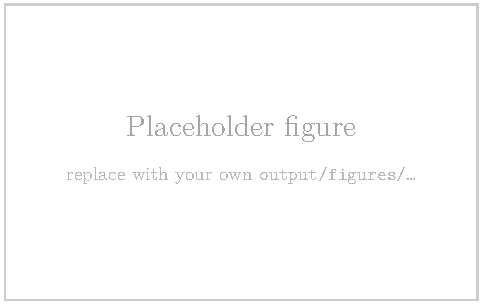
\includegraphics[width=2in]{../../assets/placeholders/placeholder-figure.pdf}
			\end{figure}		

		\onslide<2>
			\vskip2.75ex
			\begin{figure}[htp]
				\centering
				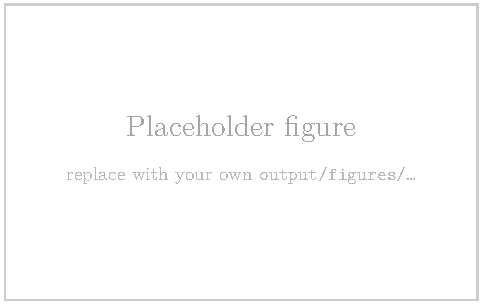
\includegraphics[width=2in]{../../assets/placeholders/placeholder-figure.pdf}
			\end{figure}											

	\end{overprint}		
\end{frame}

% THIS PAPER
\begin{frame}{This paper}
	\blockhead*{Motivation}
	\begin{itemize}
		\item Many people have ``an'' idea of North
		\item But little real experiences of it
	\end{itemize}

	\blockhead{Question}
	\begin{itemize}
		\item What is living in the North actually like?
		\begin{itemize}
			\item Some point
			\item Another point
		\end{itemize}
		\item Where does the idea of North start and end?
	\end{itemize}

	\blockhead{Approach}
	\begin{itemize}
		\item Interview five people who have had direct exposures to the North
		\item Build and estimate model of Northern migration
	\end{itemize}
\end{frame}


% THIS PAPER
\begin{frame}{Preview of findings}
	\begin{enumerate}
		\setlength\itemsep{\slideitemgap}
		\item Finding 1
		\item Finding 2
		\item Finding 3
	\end{enumerate}
\end{frame}

\section*{Literature}

\begin{frame}[label=literature]{Literature}
	\begin{enumerate}
		\setlength\itemsep{0.5em}

		% ASYMMETRIC INFORMATION
		\item \text{\textbf<2>{Asymmetric information and signaling}}
			\only<2> {
			\begin{scriptsize}
				\item[] Quality uncertainty: \textcolor{hex666666}{\citet*{Akerlof-1970-QJE}} Signaling: \textcolor{hex666666}{\citet*{Spence-1973-QJE}} Search and information: \textcolor{hex666666}{\citet*{Stigler-1961-JPE}}
			\end{scriptsize}
			}
			\onslide<2-> {
			\begin{scriptsize}
				\item[] \textbf{Contribution:} A tractable extension that \textcolor{hexred}{ties markups to observable group-level demand elasticities}
			\end{scriptsize}
			}
		\vskip\slideblockgap

		% PRICING AND MARKET STRUCTURE
		\item \text{\textbf<3>{Price adjustment, hedonics, and market structure}}
			\only<3> {
			\begin{scriptsize}
				\item[] Price adjustment: \textcolor{hex666666}{\citet*{Diamond-1971-JET}} Hedonic pricing: \textcolor{hex666666}{\citet*{Rosen-1974-JPE}} Labor market shocks: \textcolor{hex666666}{\citet*{Card-1990-ILRR}}
			\end{scriptsize}
			}
			\onslide<4-> {
			\begin{scriptsize}
				\item[] \textbf{Contribution:} \textcolor{hexred}{Distributional analysis} accounting for group-level cost and demand heterogeneity
			\end{scriptsize}
			}
	\end{enumerate}
\end{frame}

\section*{Background}

\begin{frame}{Background}	
	TBD. 	
\end{frame}
\section*{Data}

\begin{frame}{Data}	
	TBD. 	
\end{frame}
\section*{TOC}

\begin{frame}[noframenumbering,c]{Roadmap}
	\tableofcontents	
\end{frame}
%%%%% SEC: EMPIRICS
\section{Empirics: Interviews}
\begin{frame}[noframenumbering,c]{Roadmap}
	\tableofcontents[currentsection]
\end{frame}

% SUBSEC:
\subsection{The Northern expedition of 1882}

\begin{frame}{The Northern expedition of 1882}	
	TBD. 	
\end{frame}

% SUBSEC:
\subsection{Glenn Gould's idea of North}

\begin{frame}{Glenn Gould's idea of North}
	TBD.
\end{frame}

% SUBSEC:
\subsection{The U.S. price-to-rent ratio}

\begin{frame}{A figure on a slide}
	\centering
	% Placeholder shipped with the template (assets/placeholders/). Root-anchored path:
	% ../../ climbs from writing/slides/ to the repo root. Swap for your own output/... .
	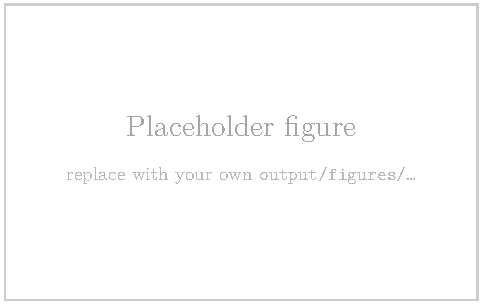
\includegraphics[width=0.5\textwidth]{../../assets/placeholders/placeholder-figure.pdf}

	{\footnotesize Placeholder. Replace the path with an \texttt{output/figures/...}
	artifact and write your own note and \textit{Source:} here.}
\end{frame}

\begin{frame}{A table on a slide}
	\centering
	% Placeholder booktabs fragment shipped with the template (assets/placeholders/).
	% Root-anchored path: ../../ climbs from writing/slides/ to the repo root. The house
	% \input pattern; \small keeps a multi-panel fragment on one slide. Swap for your own.
	\small
	% placeholder-table.tex — a neutral booktabs fragment shipped with the template.
%
% A bare tabular in the house style (\doublerule top, \midrule rules), matching what
% code/analysis exports. The demo \housetable/\input calls in writing/ point here on a
% freshly scrubbed project so the docs compile before any real table exists. Replace with
% your own output/tables/... and repoint the doc.
\begin{tabular}{l*{3}{c}}
\doublerule
                &      (1)&      (2)&      (3)\\
\midrule
Row A           &    0.000&    0.000&    0.000\\
Row B           &    0.000&    0.000&    0.000\\
Row C           &    0.000&    0.000&    0.000\\
\midrule
\end{tabular}


	\vskip\slideblockgap
	{\footnotesize Placeholder. Replace the path with an \texttt{output/tables/...}
	fragment and write your own note here.}
\end{frame}

%%%%% SEC: MODEL
\section{Model}
\begin{frame}[noframenumbering,c]{Roadmap}
	\tableofcontents[currentsection]
\end{frame}

% SUBSEC: MODEL LAYOUT
\begin{frame}{A Model of XYZ}	
	TBD. 	
\end{frame}

% SUBSEC: ESTIMATION
\subsection{Estimation}

\begin{frame}{Estimation}
	TBD. 	
\end{frame}

% SUBSEC: RESULTS
\subsection{Model results}

\begin{frame}{Model results}
	TBD. 	
\end{frame}
%%%%% SEC: CONCLUSION
\section*{Conclusion}

\begin{frame}{Conclusion}
	\begin{enumerate}
		\setlength\itemsep{\slideitemgap}
		\item Concluding remark 1
		\item Concluding remark 2
		\item Concluding remark 3
	\end{enumerate}				
\end{frame}


%%%%% THANK YOU
% Set exactly like the title page (supp/preamble-slides.tex, "customize title page"):
% same top space, the heading in the title font (\large bold), 2em below it, then the
% contact lines as the author/institute/date block. [t], not [c], so the top space is
% fixed rather than centred.
\begin{frame}[noframenumbering,t]
	\vbox{}
	\vspace{8em}%
	\begingroup
	\centering
	\begin{beamercolorbox}[center]{title}
		\usebeamerfont{title}Thank you!\par
	\end{beamercolorbox}%
	\vskip2em\par
	\begin{beamercolorbox}[center]{author}\usebeamerfont{author}Author Name\end{beamercolorbox}
	\vskip0.25em\par
	\begin{beamercolorbox}[center]{author}\usebeamerfont{author}\href{mailto:author@example.com}{author@example.com}\end{beamercolorbox}
	\vskip0.25em\par
	\begin{beamercolorbox}[center]{author}\usebeamerfont{author}\url{https://example.com}\end{beamercolorbox}
	\endgroup
\end{frame}



%%%%%%%%%%%%%%%%%%%% APPENDIX %%%%%%%%%%%%%%%%%%%%



\appendix
\begin{frame}{Appendix 1}
	\begin{enumerate}
		\setlength\itemsep{\slideitemgap}
		\item Appendix 1
		\item Appendix 2
		\item Appendix 3
	\end{enumerate}				
\end{frame}



%%%%%%%%%%%%%%%%%%%% REFERENCES %%%%%%%%%%%%%%%%%%%%



\nobibliography{../references}



\end{document} 
